\chapter{Comparison of Available Datasets}
\label{sec:dataset_selection}

The \gls{3L-CVRP} is a well-studied problem and several datasets were published in the past, considering
different constraints and characteristics. A selection of these datasets will be compared and evaluated
in this chapter. The goal is to identify a suitable dataset for training a general \gls{CLP} classifier that can predict
the feasibility of the \gls{CLP} of single tours from different datasets. Therefore, the dataset needs
heterogeneous characterists to represent numerous possible use-cases
as shown in Chapter~\ref{sec:motivation_feasibility_prediction}. Five published \cgls{3L-CVRP} datasets are presented with respect to their overall characteristics.
Each dataset gets an unique identfier to simplify the comparison and is shown in parenthesis
after the following individual introduction. The first \cgls{3L-CVRP} dataset was published by \citeauthor{gendreau_tabu_2006} in
\citeyear{gendreau_tabu_2006} and delivered the first \cgls{3L-CVRP} instances containing huge and heavy items (\gendreauDataSet).\footcite[cf.][]{gendreau_tabu_2006}
The second dataset was published by \citeauthor{moura_integrated_2009} in \citeyear{moura_integrated_2009},
and combines the \gls{VRP} from \citeauthor{solomon_algorithms_1987} and the \gls{CLP} instances from
\citeauthor{bischoff_issues_1995} defining the \gls{3L-VRPTW} considering
many items of small size and weight (\mouraDataSet).\footcites[cf.][]{solomon_algorithms_1987,bischoff_issues_1995}[][]{moura_integrated_2009}
The first dataset containing real-life data was published by \citeauthor{ceschia_local_2013} in \citeyear{ceschia_local_2013}
and contains the instances with the most items considered (\ceschiaDataSet).\footcite[cf.][]{ceschia_local_2013}
Krebs published two different datasets in
\citeyear{krebs_advanced_2021} with a focus on more realistic constraints. The first one contains a set
of realistic constraints and offers a wide range of instance sizes (\krebsADataSet).\footcite[cf.][]{krebs_advanced_2021}
The second one focuses on semi-trailer trucks and special requirements for axle weights (\krebsBDataSet).\footcite[cf.][]{krebs_axle_2021}
The characteristics of the datasets are summarized in the following Table~\ref{tab:dataset_comparison},
where the brackets [\,] indicate a range of possible values and the braces $\{\,\}$ symbolizes tuples of geometric dimensions.
Here, \textit{relative} relates to the ratio of item properties to the vehicle capacity or dimensions,
and a \textit{item type} is defined by its geometrical dimensions, the weight, and possible stability characteristics, such as fragility or \gls{LBS}.
When the number of item types is smaller than the number of items, items with equal type occur multiple times.

\newcolumntype{C}[1]{>{\centering\arraybackslash}p{#1}}
\newcolumntype{L}[1]{>{\raggedright\arraybackslash}p{#1}} % left-aligned
\begin{table}[ht]
    \centering
    \small
    \renewcommand{\arraystretch}{1.1}   % a touch more row height
    \begin{tabular}{@{}lccccc@{}}
        \toprule
        \textbf{Dataset} & \textbf{Instances} & \textbf{Customers} & \textbf{Agg. Mass}\footnote{Average is based on all customers of the instances.} & \textbf{Agg. Vol.} \footnotemark[\value{footnote}]       & \textbf{Agg. Items}\footnotemark[\value{footnote}] \\
        \midrule
        \gendreauDataSet & 27                 & [15, 100]          & 0.137                                                                            & 0.127                                                    & 2.00                                               \\
        \mouraDataSet    & 46                 & 25                 & 0.077                                                                            & 0.176                                                    & 52.0                                               \\
        \ceschiaDataSet  & 13                 & [11, 129]          & 0.063                                                                            & 0.160                                                    & 18.1                                               \\
        \krebsADataSet   & 600                & [20, 100]          & 0.098                                                                            & 0.100                                                    & 4.41                                               \\
        \krebsBDataSet   & 80                 & [30, 120]          & 0.036                                                                            & 0.052                                                    & 4.00                                               \\
        \toprule
        \textbf{Dataset} & \textbf{Items}     & \textbf{Types}     & \textbf{\text{Routes}}\footnote{Average is based on the instances.}              & \textbf{\text{Route Len}}\footnotemark[\value{footnote}] & \textbf{Fragility}\footnotemark[\value{footnote}]  \\
        \midrule
        \gendreauDataSet & [26, 199]          & [26, 199]          & 6.13                                                                             & 6.22                                                     & 0.25                                               \\
        \mouraDataSet    & 1050, 1550         & 5                  & 4.40                                                                             & 6.72                                                     & 0.29                                               \\
        \ceschiaDataSet  & [254, 8060]        & [9, 97]            & 10.2                                                                             & 5.81                                                     & 0.10                                               \\
        \krebsADataSet   & 200, 400           & 3, 10, 100         & 6.77                                                                             & 13.6                                                     & 0.24                                               \\
        \krebsBDataSet   & 200, 400           & 10, 100            & 3.87                                                                             & 22.1                                                     & 0.10                                               \\
        \bottomrule
    \end{tabular}
    \caption[Numerical comparison of different 3L--CVRP Datasets.]{Numeric comparisons between five avalaible datasets.}
    \label{tab:dataset_comparison}
\end{table}

The most important consideration, when selecting a suitable dataset for the training of a classifier,
is how representative single tours from one dataset are for all other datasets. Therefore, the numeric characteristics
should not contain outliers. The \gendreauDataSetText dataset has the most extreme values for the relative mass, minimum dimension of items,
and the quantity of items per customers. The \mouraDataSetText dataset includes the highest number of lighweight items per customer,
which can not represent the other datasets. \ceschiaDataSetText contains instances with the most items and the greatest range
of item dimensions, but the relative mass per item is very low. The datasets published by Krebs
reflect average characteristics overall. Between the two datasets, \krebsADataSetText shows the better performance,
as the items in \krebsBDataSetText have very low mass.
The following Table~\ref{tab:constraint_matrix} provides an overview of the constraints considered
in each dataset showcasing the realistic profile. The constraints are categorized in the five groups introduced
in Chapter~\ref{sec:clp_definition}.
\clearpage

\begin{table}[ht]
    \centering
    \small
    \renewcommand{\arraystretch}{1.2}
    \begin{tabular}{@{}L{1.8cm}L{3cm}C{1.6cm}C{1.6cm}C{1.6cm}C{1.6cm}C{1.6cm}@{}}
        \toprule
        \textbf{Category}          & \textbf{Constraint} &                        &                     & \textbf{Dataset}      &                      &                      \\
                                   &                     & Gendreau\newline(2006) & Moura\newline(2009) & Ceschia\newline(2013) & Krebs\newline(2021a) & Krebs\newline(2021b) \\
        \midrule
        \multirow{3}{*}{Container} & Load Capacity       & $\bullet$              & $\bullet$           & $\bullet$             & $\bullet$            & $\bullet$            \\
                                   & Load Balance        &                        &                     &                       & $\bullet$            &                      \\
                                   & Axle Weights        &                        &                     &                       & $\bullet$            & $\bullet$            \\\midrule
        \multirow{3}{*}{Item}      & z-Rotation          & $\bullet$              & $\bullet$           & $\bullet$             & $\bullet$            & $\bullet$            \\
                                   & Fragility           & $\bullet$              &                     & $\bullet$             & $\bullet$            & $\bullet$            \\
                                   & LBS                 &                        &                     & $\bullet$             & $\bullet$            &                      \\\midrule
        \multirow{1}{*}{Cargo}     & Complete Shipm.     & $\bullet$              & $\bullet$           &                       & $\bullet$            & $\bullet$            \\\midrule
        \multirow{6}{*}{Position}  & Geometry            & $\bullet$              & $\bullet$           & $\bullet$             & $\bullet$            & $\bullet$            \\
                                   & Orthogonality       & $\bullet$              & $\bullet$           & $\bullet$             & $\bullet$            & $\bullet$            \\
                                   & Reachability        &                        &                     & $\bullet$             & $\bullet$            &                      \\
                                   & Sequence            & $\bullet$              &                     &                       & $\bullet$            &                      \\
                                   & LIFO                & $\bullet$              & $\bullet$           & $\bullet$             & $\bullet$            & $\bullet$            \\
                                   & MLIFO               &                        &                     & $\bullet$             & $\bullet$            &                      \\\midrule
        \multirow{2}{*}{Load}      & Robust Stability    &                        &                     & $\bullet$             & $\bullet$            &                      \\
                                   & Support Area        & $\bullet$              & $\bullet$           &                       &                      & $\bullet$            \\

        \bottomrule
    \end{tabular}
    \caption[Overview of CLP constraints in selected 3L--CVRP datasets.]{Matrix overview of constraints covered in selected datasets. A bullet ($\bullet$) indicates that the constraint is considered.}
    \label{tab:constraint_matrix}
\end{table}

This comparison shows that all datasets include similar types of constraints, but the level
of complexity varies. \krebsADataSetText and \ceschiaDataSetText stand out by incorporating
more advanced constraints such as robust stability, reachability, and \gls{LBS}, in comparison to
basic ones like support area, \gls{LIFO} and fragility. To further investigate the differences
between the datasets, Figure~\ref{fig:dataset_comparison} visualizes the relative mass and
volume of all items requested by individual customers. This representation reflects the
unconstrained lower bound on vehicle usage. For example, the \mouraDataSetText dataset includes 46
instances with 25 customers each, resulting in $25 \cdot 46 = 1150$ dots in the plot.
Additionally, the size of each scatter point indicates the total number of items requested.

\begin{figure}[ht]
    \centering
    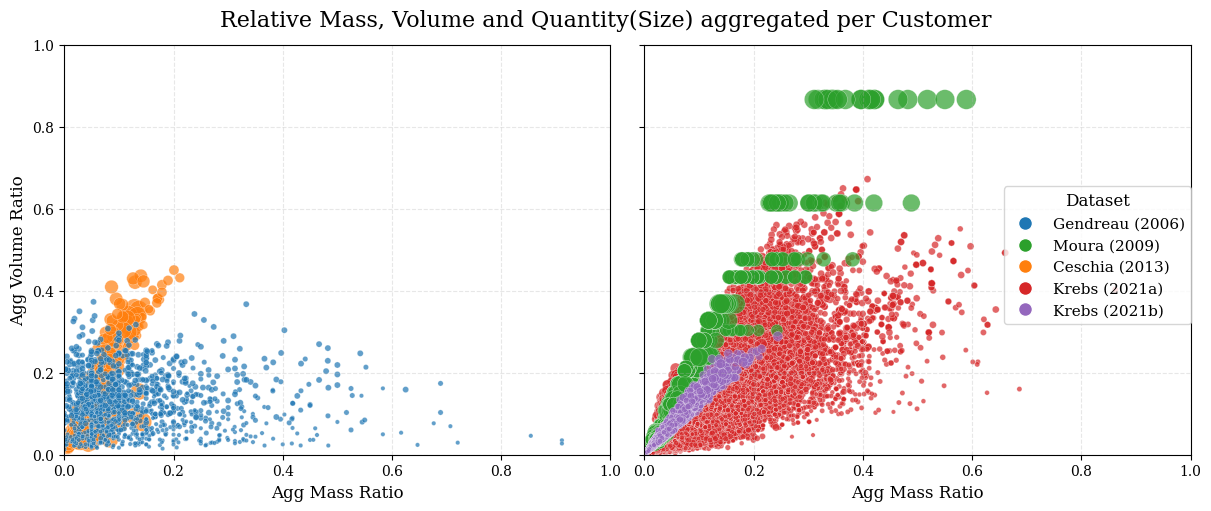
\includegraphics[width=0.85\textwidth]{pictures/comparison_datasets_3lcvrp.png}
    \caption{Comparison aggregated customer demands of different 3L--CVRP/ 3L--VRPTW datasets.}
    \label{fig:dataset_comparison}
\end{figure}

The dispersion of the data points reflects the diversity of individual instances in terms of volume
and mass dependency. A more balanced profile suggests that some customers tend to order items that
are either mass- or volume-intensive, which supports training the model on more heterogeneous data.
Therefore, the dataset should cover a wide range of cases, varying in mass, volume, and item
quantity per customer. The widest spread is observed in \krebsADataSetText and \gendreauDataSetText serving
both as good dataset candidates for training a classifier. In the overall comparison the \krebsADataSetText dataset
is selected as the most suitable and the properties of this dataset will be further investigated.
The dataset \krebsADataSetText contains 18 different instance types resulting from the combinations
of number of customers, item types and items. The following Figure~\ref{fig:krebs_dataset_analysis_detailes} plots
the relative mass and volume of all items requested by individual customers for each of the 18 instances.

\begin{figure}[ht]
    \centering
    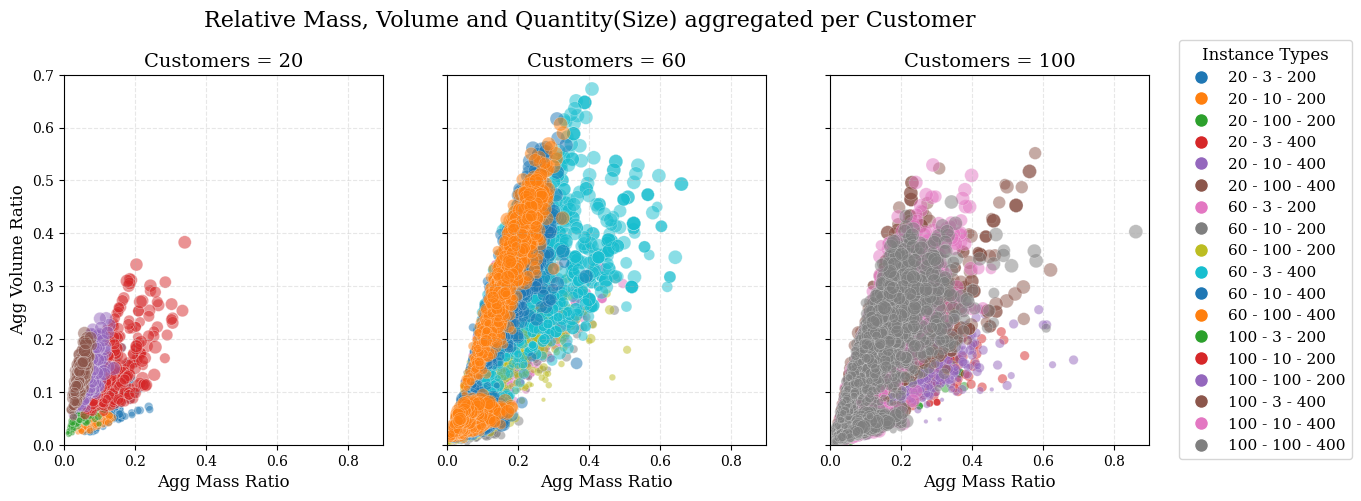
\includegraphics[width=0.85\textwidth]{pictures/krebs_instances_detailed.png}
    \caption[Visualization of different instances of \textcite{krebs_advanced_2021} dataset.]{Visualization of different instances of \krebsADataSetText dataset.
        The instances are named by the number of customers, item types and items.}
    \label{fig:krebs_dataset_analysis_detailes}
\end{figure}

Several insights can be obtained from the analysis of this plot. Firstly, the aggregated relative
volume and mass per customer is significantly lower than for the instances with 60 or 100 customers. Secondly,
the distribution differs from each instance type, ranging from quite linear distributions in a narrow
interval (e.g. instance 60-100-400) to quite broad distributions (e.g. instance 100-100-400). These two observations need to be considered, when selecting
instances to generate training data for the classifier to avoid a homogenous training set, and
as a consequence poor classifying results with a low accuracy.




%\section{Overview of Public Datasets}
%\section{Evaluation Criteria: Diversity, Realism, Labeling, Size}
%\section{Comparison of Selected Datasets}
%\section{Justification for Dataset Selection}

\begin{comment}
The \gendreauDataSetText dataset contains the relative heaviest items, whereas the other datasets with the exception of
\krebsADataSetText contains lightweight items. The quanitity of ordered items per customer differs the most between
the \gendreauDataSetText and the \mouraDataSetText datasets, and represents the most lowest and the highest values
respectively.
\end{comment}